\subsection{Propriedades do Conjunto Típico}
\begin{frame}%[allowframebreaks]
  \frametitle{Propriedades do Conjunto Típico}
  \begin{theorem}[Propriedades do Conjunto Típico $A_\epsilon^{(n)}$]
  \begin{enumerate}
  \item Se $(x_1, x_2, \ldots, x_n) \in A_\epsilon^{(n)}$, então
        \begin{equation}
        H(X) - \epsilon \leq - \frac{1}{n} \log p(x_1, x_2, \ldots, x_n) \leq H(X) + \epsilon
        \end{equation}
  \item $p(A_\epsilon^{(n)}) = p\left( \left\{ x: x \in A_\epsilon^{(n)} \right\} \right) > 1 - \epsilon$ para $n$ grande suficiente, para todo $\epsilon > 0$.
  \item Limite superior: $\vert A_\epsilon^{(n)} \vert \leq 2^{n(H(X)+\epsilon)}$, onde $\vert A_\epsilon^{(n)} \vert$ é o número de elementos no conjunto $A_\epsilon^{(n)}$.
  \item Limite inferior: $\vert A_\epsilon^{(n)} \vert \geq (1-\epsilon) 2^{n(H(X) - \epsilon)}$ para $n$ grande suficiente.
  \end{enumerate}
  \end{theorem}

  \begin{itemize}
  \item O conjunto típico possui, essencialmente, probabilidade $1$ (algo típico irá tipicamente ocorrer).
  \item Todos os itens neste conjunto terão a mesma probabilidade $\approx 2^{-nH}$.
  \end{itemize}
\end{frame}

\begin{frame}%[allowframebreaks]
  \frametitle{Exemplo $K=\vert \{0,1\} \vert$: Conjunto Típico}
  \begin{itemize}
  \item Suponha o Ensaio de Bernoulli com distribuição uniforme, $K=2$, 
        $\mathcal{X} = \{0,1\}$, $p=0.5$, entropia $H=1$ e
        $\vert A_\epsilon^{(n)} \vert = 2^{nH} = 2^n = K^n$, 
        então todas as sequências ocorreram com igual probabilidade.
  \item Considere agora uma distribuição não-uniforme, $p=0.1$ e $q=1-p=0.9$, a entropia será
        $H\approx 0.469$. Considere $n=100$, então 
        $K^{100} = 2^{100} = 10^{\log_{10} 2^{100}} \approx 10^{100 \times 0.30103} \approx 10^{30}$,
        a capacidade representacional das sequencias da fonte. 
        Mas $\vert A_\epsilon^{(n)} \vert = 2^{nH} = 10^{nH \times \log_{10} 2} \approx 10^{14} \ll 10^{30} \approx K^{100}$. 
        O número de sequências típicas é muito menor que o número de possíveis sequências.
  \item Ineficiência: capacidade representacional é muito maior do que as coisas que ocorrem.
        O alfabeto da fonte é pobre para realizar compressão.
  \item Assuma $\epsilon$ muito pequeno, então onde foi parar a massa das $\approx 10^{30} - 10^{14}$ 
        sequencias? (veremos adiante)
  \end{itemize}
\end{frame}


\begin{frame}%[allowframebreaks]
  \frametitle{Conjunto Típicos são Típicos}
  \begin{itemize}
  \item Pela definição
        \begin{equation}
        p(A_\epsilon^{(n)}) > 1 - \epsilon \text{ para qualquer } \epsilon > 0
        \end{equation}
  \item Então $A_\epsilon^{(n)}$ possui praticamente toda probabilidade, e cada elemento
        em $A_\epsilon^{(n)}$ possui a mesma probabilidade, então
        \begin{equation}
        p(x) \approx 2^{-nH} \forall x \in A_\epsilon^{(n)}
        \end{equation}
  \item Exemplo: Ensaio de Bernoulli $X_i \sim \text{Bernoulli}(p)$ com 
        $p(X_i = 1) = p = 1 - p(X_i = 0)$ e $p>0.5$.
  \item Probabilidade de $n$ $1$s sucessivos é $p^n$ e esta é a sequência mais provável.
  \item Probabilidade de uma sequência típica é $2^{-nH}$.
  \item Para $n=100$, $p-0.9 = 1 - q$, a sequência mais provável possui probabilidade
        $p^n \approx 2.66 \times 10^{-5}$, mas uma sequencia típica possui probabilidade
        $2^{-nH} \approx 7.62 \times 10^{-15}$.
  \end{itemize}
\end{frame}

\begin{frame}%[allowframebreaks]
  \frametitle{Exemplo $K=\vert \{0,1\} \vert$: Conjunto Típico}
  \begin{itemize}
  \item Suponha o Ensaio de Bernoulli com distribuição uniforme, $K=2$, 
        $\mathcal{X} = \{0,1\}$, $p=0.5$, entropia $H=1$ e
        $\vert A_\epsilon^{(n)} \vert = 2^{nH} = 2^n = K^n$, 
        então todas as sequências ocorreram com igual probabilidade.
  \item Considere agora uma distribuição não-uniforme, $p=0.1$ e $q=1-p=0.9$, a entropia será
        $H\approx 0.469$. Considere $n=100$, então 
        $K^{100} = 2^{100} = 10^{\log_{10} 2^{100}} \approx 10^{100 \times 0.30103} \approx 10^{30}$,
        a capacidade representacional das sequencias da fonte. 
        Mas $\vert A_\epsilon^{(n)} \vert = 2^{nH} = 10^{nH \times \log_{10} 2} \approx 10^{14} \ll 10^{30} \approx K^{100}$. 
        O número de sequências típicas é muito menor que o número de possíveis sequências.
  \item Ineficiência: capacidade representacional é muito maior do que as coisas que ocorrem.
        O alfabeto da fonte é pobre para realizar compressão.
  \item Assuma $\epsilon$ muito pequeno, então onde foi parar a massa das $\approx 10^{30} - 10^{14}$ 
        sequencias? (veremos adiante)
  \end{itemize}
\end{frame}

\begin{frame}%[allowframebreaks]
  \frametitle{Conjunto Típicos são Típicos}
  \begin{itemize}
  \item Pela definição
        \begin{equation}
        p(A_\epsilon^{(n)}) > 1 - \epsilon \text{ para qualquer } \epsilon > 0
        \end{equation}
  \item Então $A_\epsilon^{(n)}$ possui praticamente toda probabilidade, e cada elemento
        em $A_\epsilon^{(n)}$ possui a mesma probabilidade, então
        \begin{equation}
        p(x) \approx 2^{-nH} \forall x \in A_\epsilon^{(n)}
        \end{equation}
  \item Exemplo: Ensaio de Bernoulli $X_i \sim \text{Bernoulli}(p)$ com 
        $p(X_i = 1) = p = 1 - p(X_i = 0)$ e $p>0.5$.
  \item Probabilidade de $n$ $1$s sucessivos é $p^n$ e esta é a sequência mais provável.
  \item Probabilidade de uma sequência típica é $2^{-nH}$.
  \item Para $n=100$, $p-0.9 = 1 - q$, a sequência mais provável possui probabilidade
        $p^n \approx 2.66 \times 10^{-5}$, mas uma sequencia típica possui probabilidade
        $2^{-nH} \approx 7.62 \times 10^{-15}$.
  \end{itemize}
\end{frame}

\begin{frame}%[allowframebreaks]
  \frametitle{Sequencias Não-Típicas não são típicas}
  \begin{itemize}
  \item $p^n \gg 2^{-nH}$: a sequência mais provável é muito mais provável do que uma 
        sequencia típica.
  \item O que ocorre com a probabilidade da sequencia mais provável, na média (por símbolo),
        quando $n$ cresce
        \begin{equation}
        - \frac{1}{n} \log p^n = - \log p = \log 1/p \xrightarrow[n \rightarrow \infty] p H ?
        \end{equation} 
  \item O conjunto típico possui, essencialmente, toda a probabilidade $p(A_\epsilon^{(n)}) > 1 - \epsilon $.
  \item A sequencia mais provável está no conjunto típico? 
        Não, já que a probabilidade da sequencia mais provável não é $2^{-nH}$.
  \item $n=100$, $p=0.9=1-q$. Considere uma sequência com noventa $1$s e dez $0$s.
        A probabilidade é $p^{90}(1-p)^{10} \approx 7.62 \times 10^{-15} \approx 2^{-nH}$.
  \item Esta sequencia muito improvável é típica.
  \end{itemize}
\end{frame}

\begin{frame}%[allowframebreaks]
  \frametitle{Probabilidade Média de Sequencias}
  \begin{itemize}
  \item Pela PEA (Propriedade da Equipartição Assintótica), temos que se 
        $(x_1, \ldots, x_n)$ é típico (i.e., $(x_1, \ldots, x_n) \in A_\epsilon^{(n)}$, 
        para qualquer $\epsilon > 0$), então
        \begin{equation}
        - \frac{1}{n} \log p(x_1, \ldots, x_n) \xrightarrow[n \rightarrow \infty]{p} H 
        \end{equation}
  \item Para as sequencias mais prováveis, quando $n$ é grande suficiente, teremos (para $p>0.5$)
        \begin{equation}
        - \frac{1}{n} \log p^n = - \log p = \log 1/p \xrightarrow[n \rightarrow \infty]{p} - \log p
        \end{equation}
  \item A probabilidade média da sequencia mais provável é bem diferente da sequencia típica.
  \end{itemize}
\end{frame}

\begin{frame}%[allowframebreaks]
  \frametitle{Sequencias Típicas}
  \begin{itemize}
  \item o conjunto típico possui essencialmente toda da probabilidade.
  \item Como pode uma sequencia com a maior probabilidade não ser típica,
        mas uma sequência com probabilidade muito menor ser típica?
  \item Existe um número exponencialmente crescente de sequencias típicas, cada uma
        com probabilidade menor do que a sequencia de maior probabilidade.
  \item A probabilidade individual de cada sequencia vai a zero quando $n$ cresce.
  \item O tamanho do conjunto típico cresce rapidamente, quando $n \rightarrow \infty$,
        de forma que a probabilidade de $A_\epsilon^{(n)}$ vai a $1$.
  \item O tamanho do conjunto das sequencias muito prováveis cresce lentamente, de forma
        que a probabilidade do conjunto vai a zero quando $n \rightarrow \infty$. 
  \end{itemize}
\end{frame}

\begin{frame}[allowframebreaks]
  \frametitle{Sequencias Típicas} 
  A probabilidade de uma sequência $x_{1:n}$, onde $x_i \in \mathcal{X} = \{a_1, \ldots, a_K\}$, é dada por
  \begin{equation}
  P(x_{1:n}) = P(x_1) P(x_2) \ldots P(x_n) \approx p_1^{p_1 n} p_2^{p_2 n} \ldots p_K^{p_K n} ,
  \end{equation}
  onde consideramos que, em uma sequência muito longa, esperamos observar $p_1 n$ ocorrências do símbolo $a_1$,
  $p_2 n$ ocorrências do símbolo $a_2$, etc.

  A informação associada a esta sequência típica é
  \begin{eqnarray}
  \log \frac{1}{P(x_{1:n})} &\approx& \sum_{i=1}^K \log p_i^{-p_i n} \\
                &=& n \sum_{i=1}^K p_i \log \frac{1}{p_i} = n H(X).
  \end{eqnarray}
  Uma sequência típica terá probabilidade próxima de $2^{-n H(X)}$.

  \framebreak
  \begin{figure}[h!]
  \centering
  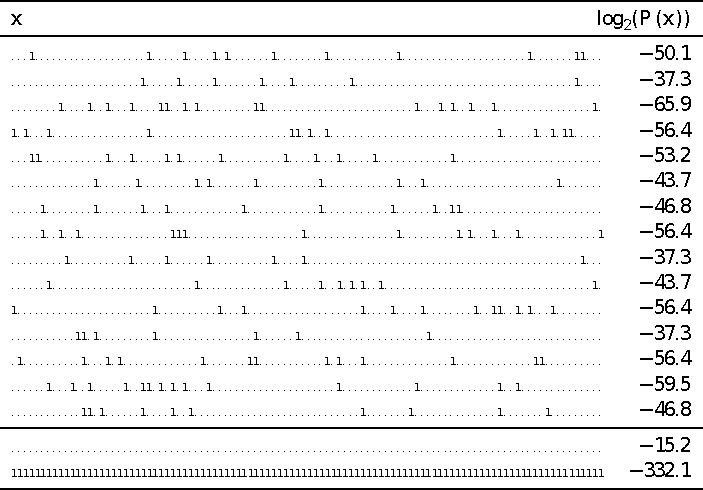
\includegraphics[width=0.5\textwidth]{images/seq100mackay.pdf}
  \caption{Sequências regadas por um ensaio de Bernoulli com $n=100$ e $P(X=1) = p = 0.1$. 
        As 15 sequências superiores representam amostras típicas. As duas últimas sequências
        representam a sequência mais provável e a menos provável \cite{mackay2003}.}
  \label{fig:seq100mackay}
  \end{figure}

  \framebreak
  \begin{figure}[h!]
  \centering
  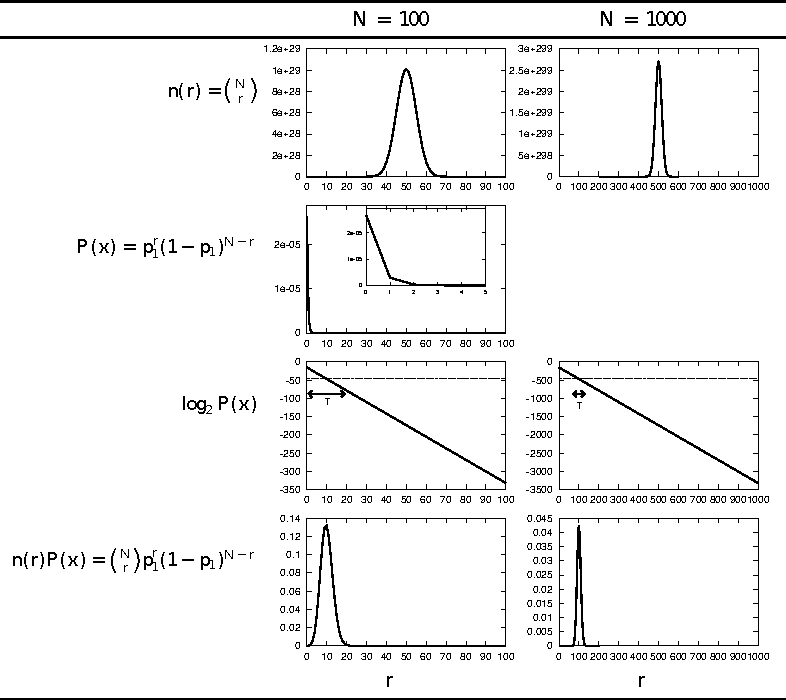
\includegraphics[width=0.5\textwidth]{images/seq100mackay2.pdf}
  \caption{Para $p=0.1$, $n=100$ e $n=1000$ os gráficos ilustram $n(r)$, o número de strings contendo
        $r$ 1s; a probabilidade $P(x_{1:n})$ para uma string contendo $r$ 1s; a mesma probabilidade
        em escala logarítmica; e a probabilidade total $n(r) P(x_{1:n})$ de todas as strings contendo $r$ 1s \cite{mackay2003}.}
  \label{fig:seq100mackay2}
  \end{figure}


  \framebreak
  \begin{figure}[h!]
  \centering
  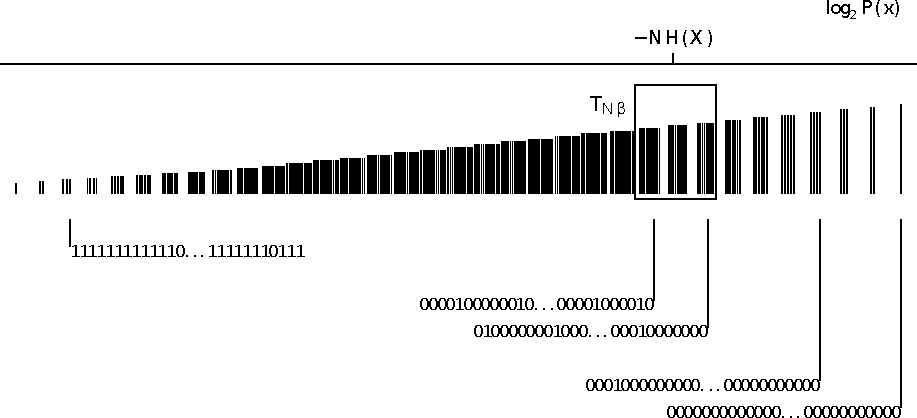
\includegraphics[width=0.5\textwidth]{images/seq100mackay3.pdf}
  \caption{Diagrama esquemático ilustrando todas as sequencias no conjunto $\mathcal{X}^n$ ordenadas pela probabilidade \cite{mackay2003}.}
  \label{fig:seq100mackay3}
  \end{figure}


  O termo \textbf{equipartição} é utilizado para descrever a ideia de que os membros do conjunto típico
  possuem aproximadamente a mesma probabilidade.

  
\end{frame}

